\documentclass[a4paper]{article}

\usepackage[pdftex]{graphicx}
\usepackage[margin=3cm]{geometry}
\usepackage{verbatim,moreverb,amssymb,amsmath}


\newcounter{question}
\newcommand{\question}{\refstepcounter{question}\section*{Question~\thequestion}}
\renewcommand*\thequestion{\arabic{question}}


\begin{document}

\pagestyle{empty}
\thispagestyle{empty}



\noindent
\begin{minipage}{\columnwidth}
  \centering
  \Large
  DA4002 (HT11) Halmstad University\\
  Introduction to Algorithms, Data Structures, and Problem Solving\\[3\baselineskip]
  \Huge
  Written Exam\\
  \Large
  Monday, October 24, 2011\\
  15h30 -- 19h30, room K{\aa}ren\\[2\baselineskip]
  Examiner: Roland Philippsen (phone 7249)
\end{minipage}

\vfill

\noindent
\begin{center}
\fbox{
  \begin{minipage}{0.8\columnwidth}
    \textbf{Student Name:}\\[3\baselineskip]
  \end{minipage}
}
\end{center}

\vfill



\section*{Rules}

Aside from the obvious rules of conduct exams (e.g.\ no chatting):

\begin{itemize}
\item
  \textbf{No computing devices} (laptops, phones, calculators, \emph{etc}).
\item
  \textbf{No books or printouts}.
\item
  \textbf{Allowed self-written notes}: two sheets of A4 paper (front and back).
\end{itemize}



\section*{General Guidelines}

\begin{itemize}
\item
  \textbf{Read carefully} and pace yourself.
  You can solve the problems in any order you want, but later problems may be easier to solve after you have answered the preceding questions.
\item
  \textbf{Write clearly} and draw clear diagrams.
  If you need to correct a mistake, then cleanly cross out the wrong answer and clearly indicate where the correction can be found.
\item
  \textbf{Indicate the question number} for each of your answers.
  If a question has sub-questions, indicate the sub-question number after the main question number, separated by a dot.
  For example, question 3 has 4 sub-questions, and their answers should be numbered 3.1, 3.2, 3.3, and 3.4.
\end{itemize}



\pagebreak
\pagestyle{plain}
\thispagestyle{plain}
\setcounter{page}{1}



\question\label{q:container-structures-a}

The following four figures show four examples of data structures.
They are labeled with the letters \textbf{(A)}, \textbf{(B)}, \textbf{(C)}, and \textbf{(D)}.
The table below them lists names of data structure types.
For each type listed in the table, determine whether it is represented by one of the figures.
If there is a figure for a given type, write the corresponding letter into the second column of the table.
Mark structure types which are not shown in any diagram with a big \textbf{X}.\\[\baselineskip]

\noindent
\begin{minipage}[b]{0.44\columnwidth}
  \fbox{\textbf{(A)}\includegraphics[width=\columnwidth,trim=1cm 1cm 1cm 1cm]{fig/k-ary-tree.pdf}}
  \fbox{\textbf{(B)}\includegraphics[width=\columnwidth,trim=1cm 1cm 1cm 1cm]{fig/simply-linked-list.pdf}}
\end{minipage}
\hfill
\begin{minipage}[b]{0.5\columnwidth}
    \fbox{\textbf{(C)}\includegraphics[width=\columnwidth,trim=1cm 1cm 1cm 1cm]{fig/directed-cyclic-graph.pdf}}
    \fbox{\textbf{(D)}\includegraphics[width=\columnwidth,trim=1cm 1cm 1cm 1cm]{fig/undirected-graph.pdf}}
\end{minipage}

\begin{center}
  \begin{tabular}{|l|p{0.3\columnwidth}|}
    \hline
    \emph{container type} & \emph{A, B, C, D, or X} \\
    \hline
    & \\
    \textbf{simply} linked list & \\
    & \\
    \hline
    & \\
    \textbf{doubly} linked list & \\
    & \\
    \hline
    & \\
    \textbf{binary} tree & \\
    & \\
    \hline
    & \\
    \textbf{k-ary} tree & \\
    & \\
    \hline
    & \\
    \textbf{undirected} graph & \\
    & \\
    \hline
    & \\
    directed \textbf{acyclic} graph & \\
    & \\
    \hline
  \end{tabular}
\end{center}

\clearpage

\question
\label{q:container-structures-b}

In question~\ref{q:container-structures-a}, three of the types listed in the table are missing from the figures.
Draw a diagram for each missing type.
Clearly indicate which diagram is for which container type.
Make each diagram as similar as possible to one of the figures from question~\ref{q:container-structures-a}.

\clearpage

\question
\label{q:container-implementations}

The following Java code implements two data structures called \texttt{ContainerOne} and \texttt{ContainerTwo}.
Answer the following questions.
You can write the short answers as annotations on the source code, and use a separate sheet of paper for the ones that require more space.

\begin{enumerate}
\item
  Which container types are implemented by \texttt{ContainerOne} and \texttt{ContainerTwo}?
\item
  Draw a diagram of what each container looks like after \texttt{insert} has been called with the following sequence of values:
  5, 3, 13, -7, 3, 7, 42, 3, 6, 12, 11.
\item
  In \texttt{ContainerOne}:
  what is the role of \texttt{ContainerOne.handle}, \texttt{Node.foo}, and \texttt{Node.bar}?
  Suggest better names for these three fields.
\item
  In \texttt{ContainerTwo}:
  what is the role of \texttt{ContainerTwo.alpha}, \texttt{ContainerTwo.beta}, \texttt{Node.foo}, and \texttt{Node.bar}?
  Suggest better names for these four fields.
\end{enumerate}

\noindent\hrule\vspace{0.3\baselineskip}

\noindent
\begin{minipage}{0.95\columnwidth}
  \small
  \verbatimtabinput{Q3.java}
\end{minipage}

\clearpage

\question
\label{q:sorting-complexity}

A company sends their vice president for marketing (VPM) and their chief technology officer (CTO) to a big trade show.
Each of them collects business cards from the many people they meet.
Sitting down at the desks in their hotel rooms in the evening, they sort the received business cards alphabetically.
However, they employ different strategies:

\begin{description}
\item[The VPM]
  proceeds as follows:
  \begin{itemize}
  \item
    He places the pile of unsorted cards onto the desk to his right.
  \item
    He picks the top card from the unsorted pile and places it to his left.
  \item
    Then, he picks the next card from the unsorted pile, and places it either underneath or on top of the card on the left depending on whether the name on the new card comes before or after the name on the old card.
  \item
    He then repeatedly does the following, until the unsorted pile has vanished:
    he picks one card after another from the right, scans for its place in the sorted pile, and inserts it there.
  \end{itemize}
\item[The CTO]
  does it differently:
  \begin{itemize}
  \item
    He also starts by placing the unsorted pile on the right, but then he picks up groups of five cards, sorts each group in his hand, and places the resulting small sorted pile on the left.
    He repeats this until the unsorted pile is gone and he has many small sorted piles on the desk.
  \item
    Then, he proceeds to merge pairs of these small piles:
    he chooses a pair, sequentially picks the topmost card from either pile, whichever card comes first in alphabetical order, and thus creates a bigger sorted pile.
  \item
    When he runs out of small piles, he repeats the previous step with the freshly created bigger piles, merging them into even bigger piles.
  \item
    He repeats the pairwise merging until he has only one pile left.
  \end{itemize}
\end{description}

Assume that the VPM needs 0.4 seconds to compare two individual cards.
The CTO needs 5 seconds to sort 5 cards ``in hand,'' and 0.5 seconds for each card during the merging of two piles.
Assume that all other delays can be ignored.
Answer the following questions:

\begin{enumerate}
\item
  Develop a formula for $T_\text{VPM}(N)$ which allows to estimate the amount of time required by the VPM to sort $N$ business cards.
\item
  Give the \emph{Big-Oh} complexity for $T_\text{VPM}(N)$.
\item
  Develop a formula for $T_\text{CTO}(N)$ which allows to estimate the amount of time required by the CTO to sort $N$ business cards.
\item
  Give the \emph{Big-Oh} complexity for $T_\text{CTO}(N)$.
\item
  Who will take longer to sort small amounts of business cards ($N<20$ or so)?
  Who will take longer to sort large amounts of cards ($N>40$ or so)?
  Explain your answers!
\end{enumerate}

\clearpage

\question
\label{q:recursion-and-dp}

The number sequence $\{G_n\}$ is defined for all natural numbers $n>0$ by the following recursion.
In order to compute $G_n$, one of your friends implemented the \texttt{gRec} Java method shown in the box below the equation.
There are three \texttt{return} statements in that method, and they are labeled with the letters \textbf{(A)}, \textbf{(B)}, and \textbf{(C)}.

\begin{equation*}
  G_n =
  \begin{cases}
    0 &\text{for } n \le 2 \\
    1 &\text{for } n = 3 \\
    2G_{n-3} - G_{n-2} + G_{n-1} &\text{for } n \ge 4
  \end{cases}
\end{equation*}

\begin{center}
  \fbox{
    \begin{minipage}{0.7\columnwidth}
      \small
      \verbatimtabinput{GRec.java}
  \end{minipage}}
\end{center}

In order to validate that the \texttt{gRec} method works correctly, your friend has traced which \texttt{return} statements are encountered when \texttt{gRec} is called with \texttt{n=4}.
This execution trace is given in the table shown below:
the first column lists the value of the method argument \texttt{n},
the second column lists the label of the \texttt{return} statement which gets executed,
and the third column shows which value gets returned.
For the statement marked \textbf{(C)}, your friend helpfully also wrote down how the value gets computed.

\begin{center}
  \begin{tabular}{|c|c|l|}
    \hline
    n & label & value \\
    \hline
    1  & A & 0 \\
    2  & A & 0 \\
    3  & B & 1 \\
    4  & C & 2* 0 - 0 + 1 = 1 \\
    \hline
  \end{tabular}
\end{center}

Answer the following questions:

\begin{enumerate}
\item
  Trace the \texttt{gRec} method call for \texttt{n=6}.
  Write it down as a table that follows the same format as the table above.
\item
  Your friend notices that his implementation is really slow for \texttt{n} larger than 20 or so:
  with \texttt{n=20} it takes 0.3 seconds, but with \texttt{n=40} it takes almost a minute!
  Explain why this happens.
  If you can draw a diagram to illustrate the root cause, even better!
\item
  There are two problem solving techniques which can avoid the rapid growth of execution time in this case.
  Briefly explain each technique \emph{(you should not need more than two or three  sentences for each)}.
\item
  Apply both of these problem solving techniques to solve your friend's problem.
  Write separate code segments for each of them.
  You can use Java syntax or pseudo-code, as long as it is clear what is done in which order.
\end{enumerate}

\clearpage

\question
\label{q:graph-search}

\paragraph{Definition:}
A \textbf{topological ordering} of a directed graph is a sequence of its vertices such that, for every \emph{edge} $(U,V)$, $U$ appears before $V$ in the sequence.
Note that for any \emph{path} from $U$ to $V$, this also implies that $U$ comes before $V$ in the ordering.
In the example graph shown below, the sequence $(C,A,D,B)$ is a topological ordering.

\begin{center}
  \fbox{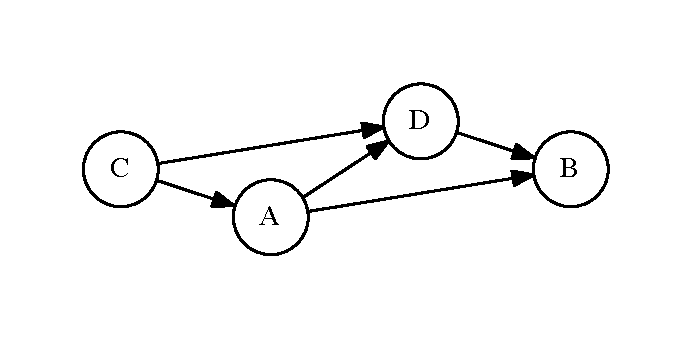
\includegraphics[width=0.3\columnwidth,trim=1cm 1cm 1cm 1cm]{fig/dag-small.pdf}}
\end{center}

\paragraph{Theorem:}
A topological ordering is possible if and only if the graph has no cycles.
In other words, a graph has to be a \textbf{directed acyclic graph} (DAG) in order to have a topological ordering.
And also, every DAG has at least one topological ordering.

\vspace{\baselineskip}
\noindent\hrule
\vspace{\baselineskip}

\noindent
Answer the following questions:

\begin{enumerate}
\item
  Prove the theorem.
\item
  Develop and describe an algorithm to detect whether a given directed graph has a cycle, based on the above theorem.\\
  \textbf{Hints:}
  \begin{itemize}
  \item
    The \emph{indegree} of a vertex $V$ is the number of incoming edges.
    In the above example, the indegree of $D$ is two.
    %%    Thus, if there is some vertex $U$ that connects to $V$, then the indegree of $V$ is at least one.
  \item
    If $V$ has an indegree equal to zero, then it can only have \emph{outgoing} paths.
    This means that $V$ cannot be on a cycle.
    In the above example, $C$ is such a vertex.
  \item
    If we remove an edge $(V,W)$, then the indegree of $W$ is decreased by one.
    If $V$ is \emph{not} on a cycle, and the removal of $(V,W)$ makes the indegree of $W$ drop to zero, then $W$ also cannot be on a cycle.
  \end{itemize}
\item
  Apply your algorithm to the two graphs shown below.
  Illustrate each step of your algorithm with a little diagram.
  Annotate each diagram with a short sentence about what has changed since the previous diagram.
  At the end of each sequence of diagrams, clearly state whether the graph has a cycle, and how this is determined by looking at the last diagram.
\end{enumerate}

\begin{center}
  \fbox{
    \begin{minipage}{0.35\columnwidth}
      \centering
      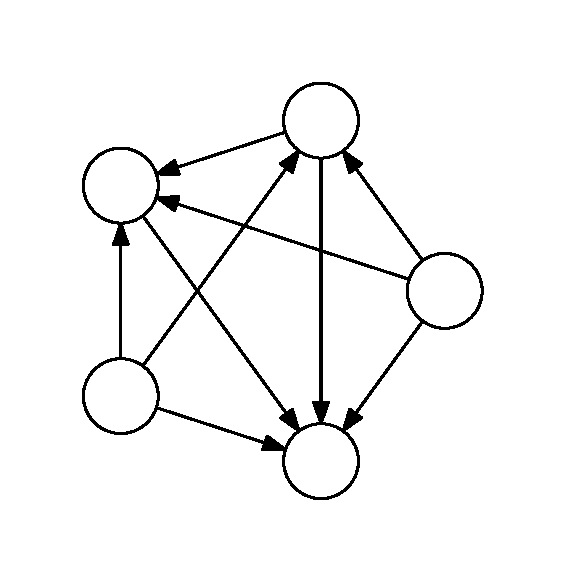
\includegraphics[width=\columnwidth,trim=1cm 1cm 1cm 1cm]{fig/cycle-detection-dag.pdf}
      \textbf{graph A}
    \end{minipage}}
  \fbox{
    \begin{minipage}{0.35\columnwidth}
      \centering
      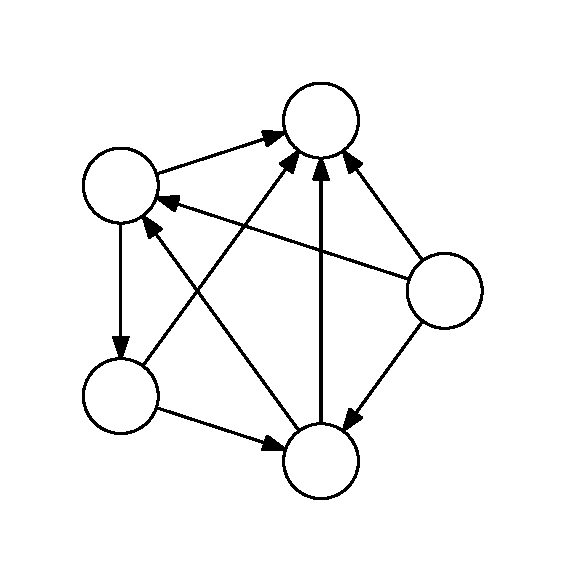
\includegraphics[width=\columnwidth,trim=1cm 1cm 1cm 1cm]{fig/cycle-detection-non-dag.pdf}
      \textbf{graph B}
    \end{minipage}}
\end{center}



\end{document}
